%=====================================================================
%  DATA SCIENCE -- Lecture 5 (final): From Patterns to Predictions
%  A First Machine-Learning Model
%  Undergraduate CSE, 40-minute lecture
%
%  Theme:  "Ink on Ivory" -- reused verbatim from Lectures 1-4. Same
%          documentclass, palette, fonts, frametitle, footer, diagram
%          language, custom commands, and the Lecture 3 code panels.
%
%  Data:   every output shown was produced by running the commands on
%          class.csv (14 students, delivered next to this file) with
%          pandas + scikit-learn. The train/test split uses
%          random_state=6, so the results reproduce exactly.
%
%  Compile:  pdflatex cse433_5.tex   (run twice)
%
%  Speaker notes are written with \note{...}. They are HIDDEN by
%  default -- uncomment one line in the SPEAKER NOTES block below.
%=====================================================================
\documentclass[aspectratio=169,11pt]{beamer}

\usepackage[T1]{fontenc}
\usepackage[utf8]{inputenc}
\usepackage{booktabs}
\usepackage{colortbl}   % coloured table rules
\usepackage{tikz}
\usepackage{pgfplots}
\pgfplotsset{compat=1.18}
\usetikzlibrary{arrows.meta,positioning,shapes.geometric,fit,calc,shadows}

% --- typography (all guarded, so the file builds on minimal installs)
\IfFileExists{charter.sty}{\usepackage{charter}}{}          % serif: Charter
\IfFileExists{helvet.sty}{\usepackage[scaled=0.92]{helvet}}{}% sans: Helvetica
\renewcommand{\familydefault}{\sfdefault}                    % body = sans
\IfFileExists{microtype.sty}{\usepackage[letterspace=140]{microtype}}{%
  \providecommand{\lsstyle}{}}

%---------------------------------------------------------------------
%  SPEAKER NOTES  (uncomment exactly one to show notes)
%---------------------------------------------------------------------
%\setbeameroption{show notes}                       % notes on separate pages
%\setbeameroption{show notes on second screen=right}% dual-screen presenting
%\setbeameroption{show only notes}                  % print notes only

%---------------------------------------------------------------------
%  PALETTE
%---------------------------------------------------------------------
\definecolor{paper}{RGB}{250,247,241}   % warm ivory  -- canvas
\definecolor{ink}{RGB}{29,43,51}        % deep ink    -- text, solid blocks
\definecolor{terra}{RGB}{181,87,60}     % terracotta  -- primary accent
\definecolor{sage}{RGB}{79,124,113}     % muted sage  -- flow, secondary
\definecolor{ochre}{RGB}{185,138,46}    % ochre       -- highlight
\definecolor{stone}{RGB}{138,129,118}   % warm gray   -- captions

%---------------------------------------------------------------------
%  THEME
%---------------------------------------------------------------------
\usetheme{default}
\usefonttheme{professionalfonts}
\setbeamertemplate{navigation symbols}{}
\setbeamercolor{background canvas}{bg=paper}
\setbeamercolor{normal text}{fg=ink}
\setbeamercolor{structure}{fg=terra}
\setbeamersize{text margin left=1.0cm,text margin right=1.0cm}

% kicker line shown above every frame title
\newcommand{\kick}{}
\newcommand{\kickx}{}
\newcommand{\setkick}[1]{\renewcommand{\kick}{#1}\renewcommand{\kickx}{}}
% step slides: text kicker + six progress dots (kept out of \MakeUppercase)
\newcommand{\setstep}[1]{\setkick{Step #1 of 6}\renewcommand{\kickx}{\stepdots{#1}}}

\setbeamertemplate{frametitle}{%
  \nointerlineskip
  \vspace{0.62em}%
  \begin{beamercolorbox}[wd=\paperwidth,leftskip=1.0cm,rightskip=1.0cm]{}
    {\sffamily\fontsize{7}{8}\selectfont\color{terra}\lsstyle\MakeUppercase{\kick}}%
    \hspace{0.5em}\kickx\par
    \vspace{2pt}
    {\rmfamily\fontsize{17.5}{20}\selectfont\color{ink}\insertframetitle}\par
    \vspace{4pt}
    
\begin{tikzpicture}
      \useasboundingbox (0,0) rectangle (\dimexpr\paperwidth-2cm\relax,1.4pt);
      \fill[terra] (0,0) rectangle (0.85cm,1.4pt);
      \fill[ink!14] (0.85cm,0.35pt) rectangle (\dimexpr\paperwidth-2cm\relax,1.05pt);
    \end{tikzpicture}
  \end{beamercolorbox}%
  \vspace{0.15em}
}

% footer: slide number + hairline progress bar
\newlength{\dsbar}
\setbeamertemplate{footline}{%
  \setlength{\dsbar}{\dimexpr\paperwidth*\insertframenumber/\inserttotalframenumber\relax}%
  \hbox{\hfill{\sffamily\fontsize{7}{8}\selectfont\color{stone}%
    \insertframenumber}\hspace{1.0cm}}%
  \vspace{1.6mm}%
  \hbox{
\begin{tikzpicture}
    \useasboundingbox (0,0) rectangle (\paperwidth,1.3pt);
    \fill[ink!10] (0,0) rectangle (\paperwidth,1.3pt);
    \fill[terra] (0,0) rectangle (\dsbar,1.3pt);
  \end{tikzpicture}}%
}

%---------------------------------------------------------------------
%  DIAGRAM LANGUAGE
%---------------------------------------------------------------------
\tikzset{
  card/.style={
    rounded corners=1.5pt, fill=white, draw=ink!14, line width=0.4pt,
    text=ink, align=center, inner sep=6pt, minimum height=0.9cm,
    font=\small,
    drop shadow={shadow xshift=0.5pt, shadow yshift=-0.9pt,
                 opacity=0.10, fill=ink}},
  soft/.style={card, fill=sage!8, draw=sage!30},
  warm/.style={card, fill=ochre!12, draw=ochre!40, text=ochre!55!black},
  solid/.style={card, fill=ink, draw=ink, text=paper, font=\small\bfseries},
  flat/.style={rounded corners=1.5pt, fill=white, draw=ink!14,
    line width=0.4pt, text=ink, align=center, inner sep=6pt,
    minimum height=0.9cm, font=\small},
  flatsoft/.style={flat, fill=sage!8, draw=sage!30},
  flatsolid/.style={flat, fill=ink, draw=ink, text=paper, font=\small\bfseries},
  ghost/.style={rounded corners=1.5pt, fill=white, draw=ink!14,
    line width=0.4pt, text=ink, align=center, inner sep=5pt, font=\footnotesize},
  flow/.style={-{Stealth[length=2.3mm,width=1.9mm]},
    draw=sage!85!ink, line width=0.7pt},
  hair/.style={draw=ink!18, line width=0.5pt},
  tag/.style={font=\scriptsize\itshape, text=stone},
  num/.style={circle, fill=terra, text=white, font=\scriptsize\bfseries,
    inner sep=0pt, minimum size=4.6mm},
  numq/.style={num, fill=ink},
  invisible/.style={opacity=0, text opacity=0},
  visible on/.style={alt={#1{}{invisible}}},
  alt/.code args={<#1>#2#3}{\alt<#1>{\pgfkeysalso{#2}}{\pgfkeysalso{#3}}},
}

% coloured accent bar along the top edge of a card
\newcommand{\accentbar}[2]{%
  \fill[#2] ([yshift=-1.8pt]#1.north west) rectangle (#1.north east);}

% six-step progress dots, used on the workflow step slides
\newcommand{\stepdots}[1]{%
  \begin{tikzpicture}[baseline=-0.55ex]
    \foreach \i in {1,...,6}{%
      \ifnum\i=#1\relax
        \fill[terra] (0.26*\i,0) circle (0.08);
      \else
        \fill[ink!22] (0.26*\i,0) circle (0.055);
      \fi}
  \end{tikzpicture}}

% large pull-quote style statement
\newcommand{\statement}[2][12.2cm]{%
  \begin{center}
  \begin{tikzpicture}
    \node[inner sep=0pt] (t) {\parbox{#1}{\centering\rmfamily #2}};
    \fill[terra] ([xshift=-0.55cm]t.north west) rectangle
                 ([xshift=-0.42cm]t.south west);
  \end{tikzpicture}
  \end{center}}

% dark statement frame
\newenvironment{darkframe}{%
  \begingroup
  \setbeamercolor{background canvas}{bg=ink}
  \begin{frame}[plain]\color{paper}}
  {\end{frame}\endgroup}

%---------------------------------------------------------------------
%  LECTURE 3 ADDITIONS  (code panels, DataFrame tables, safe fitting)
%---------------------------------------------------------------------
% monospace for code (guarded, like the other fonts)
\IfFileExists{beramono.sty}{\usepackage[scaled=0.82]{beramono}}{%
  \IfFileExists{lmodern.sty}{\renewcommand{\ttdefault}{lmtt}}{%
    \IfFileExists{courier.sty}{\usepackage{courier}}{}}}

\tikzset{
  code/.style={rounded corners=1.5pt, fill=ink, draw=ink, line width=0.4pt,
    text=paper, align=left, inner sep=7pt, font=\ttfamily\footnotesize},
  out/.style={card, align=left, inner sep=7pt, font=\ttfamily\footnotesize},
}

% inline code
\newcommand{\cd}[1]{{\ttfamily #1}}
% small spaced label sitting above a panel:  \lab{node}{TEXT}
\newcommand{\lab}[2]{%
  \node[anchor=south west, inner sep=0pt, text=stone,
        font=\sffamily\fontsize{6.5}{8}\selectfont]
    at ([yshift=2.5pt]#1.north west) {\lsstyle #2};}

% \fitin{max width}{max height}{content}: shrinks content only if it is
% too large, so nothing can run off the slide whatever fonts are installed
\newsavebox{\fitbox}
\newcommand{\fitin}[3]{%
  \sbox{\fitbox}{#3}%
  \ifdim\wd\fitbox>#1\relax
    \sbox{\fitbox}{\resizebox{#1}{!}{\usebox{\fitbox}}}\fi
  \ifdim\dimexpr\ht\fitbox+\dp\fitbox\relax>#2\relax
    \sbox{\fitbox}{\resizebox*{!}{#2}{\usebox{\fitbox}}}\fi
  \usebox{\fitbox}}

% --- the prediction dataset (class.csv), pandas-style
\newcommand{\ix}[1]{\textcolor{stone}{#1}}
\newcommand{\clsize}{\sffamily\scriptsize\renewcommand{\arraystretch}{1.05}%
  \setlength{\tabcolsep}{5pt}}
% a Pass / Fail chip
\newcommand{\pass}{{\color{sage!45!black}\textbf{Pass}}}
\newcommand{\fail}{{\color{terra}\textbf{Fail}}}

%---------------------------------------------------------------------
%  LECTURE 5 ADDITIONS  (decision-tree node styles)
%---------------------------------------------------------------------
\tikzset{
  qnode/.style={rounded corners=3pt, fill=ochre!14, draw=ochre!45,
    text=ochre!55!black, align=center, inner sep=7pt, font=\small\bfseries,
    minimum width=3.6cm},
  leafP/.style={rounded corners=1.5pt, fill=sage!15, draw=sage!55,
    text=sage!40!black, align=center, inner sep=6pt, font=\small\bfseries,
    minimum width=2.2cm},
  leafF/.style={rounded corners=1.5pt, fill=terra!12, draw=terra!50,
    text=terra, align=center, inner sep=6pt, font=\small\bfseries,
    minimum width=2.2cm},
  branch/.style={draw=ink!35, line width=0.7pt},
}

\begin{document}

%=====================================================================
% SLIDE 1 -- TITLE  (dark; motif: a tiny decision split)
%=====================================================================
\begingroup
\setbeamercolor{background canvas}{bg=ink}
\begin{frame}[plain]
  \begin{tikzpicture}[remember picture, overlay]
    % motif: a question splitting into two answers
    \begin{scope}[shift={($(current page.south east)+(-4.2cm,1.0cm)$)}]
      \fill[terra] (1.4,2.15) circle (0.12);
      \draw[paper!40, line width=0.7pt] (1.4,2.05) -- (0.5,1.2);
      \draw[paper!40, line width=0.7pt] (1.4,2.05) -- (2.3,1.2);
      \fill[paper!75] (0.5,1.05) circle (0.10);
      \fill[paper!75] (2.3,1.05) circle (0.10);
      \draw[paper!22, line width=0.6pt] (0.5,0.9) -- (0.5,0.35);
      \draw[paper!22, line width=0.6pt] (2.3,0.9) -- (2.3,0.35);
      \node[font=\scriptsize, text=paper!60] at (0.5,0.15) {Fail};
      \node[font=\scriptsize, text=paper!60] at (2.3,0.15) {Pass};
    \end{scope}
  \end{tikzpicture}

  \vfill
  \hspace{0.7cm}%
  \begin{minipage}{10.6cm}
    \vspace{2.5em}
    {\sffamily\fontsize{8}{10}\selectfont\color{terra}\lsstyle
     AN INTRODUCTION FOR UNDERGRADUATES}\\[0.75em]
    {\rmfamily\fontsize{44}{50}\selectfont\color{paper} Making Predictions}\\[0.45em]
    
\begin{tikzpicture}
      \fill[terra] (0,0) rectangle (1.5cm,1.6pt);
      \fill[paper!25] (1.5cm,0.4pt) rectangle (9.0cm,1.2pt);
    \end{tikzpicture}\\[0.6em]
    \vspace{2.3em}
    {\rmfamily\fontsize{18}{22}\selectfont\color{paper!75}
     Lecture 5 \;---\; A First Machine-Learning Model}\\[3.2em]
    {\sffamily\fontsize{11}{14}\selectfont\color{paper!85}
     Md.\ Owaliur Rahman}\\[0.25em]
    {\sffamily\fontsize{8}{10}\selectfont\color{terra}\lsstyle
     PRESIDENCY UNIVERSITY}
  \end{minipage}
  \vfill\vfill
  \note{%
    The last lecture --- say so, and say it warmly. Everything has pointed here.\\
    One sentence of recap of the journey: we learned what data is, got it,
    cleaned it, and explored it. One box of the Lecture 1 workflow is left:
    \emph{predict}.\\
    Promise for today: we build a real model --- the same kind of tool behind
    YouTube recommendations and bank fraud alerts --- on students they already
    know, read every line like a sentence, and end by predicting a student the
    computer has never seen. No maths. Then we close the course.}
\end{frame}
\endgroup

%=====================================================================
% SLIDE 2 -- THE WHOLE JOURNEY, ONE BOX LEFT                  (3 min)
%=====================================================================
\begin{frame}[plain]
  \vspace{0.3em}
  \begin{center}
    {\sffamily\fontsize{8}{10}\selectfont\color{terra}\lsstyle
     WHERE WE ARE IN THE JOURNEY}
  \end{center}
  \vspace{0.6em}
  \begin{center}
  \fitin{13.6cm}{3.6cm}{%
  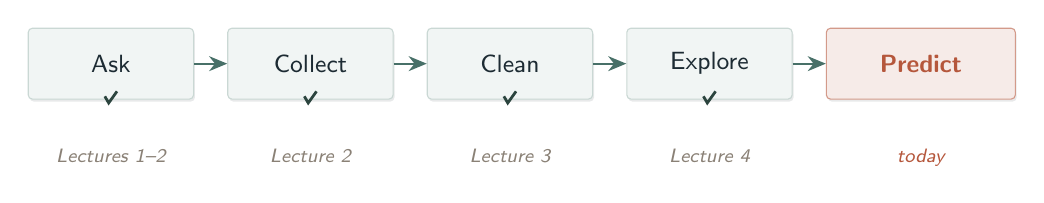
\begin{tikzpicture}[node distance=0.42cm]
    \node[soft, minimum width=2.1cm] (q) {Ask};
    \node[soft, right=of q, minimum width=2.1cm] (co) {Collect};
    \node[soft, right=of co, minimum width=2.1cm] (cl) {Clean};
    \node[soft, right=of cl, minimum width=2.1cm] (ex) {Explore};
    \node[warm, right=of ex, minimum width=2.4cm, draw=terra!60,
          fill=terra!12, text=terra] (pr) {\textbf{Predict}};
    \foreach \a/\b in {q/co,co/cl,cl/ex,ex/pr} \draw[flow] (\a) -- (\b);
    % ticks (no amssymb: draw a small check with lines)
    \foreach \n in {q,co,cl,ex}{
      \draw[sage!55!black, line width=1pt]
        ([xshift=-2.2pt,yshift=1.2pt]\n.south) -- ++(1.4pt,-2.4pt)
          -- ++(3.0pt,4.2pt);}
    \node[tag, below=0.5cm of q]  {Lectures 1--2};
    \node[tag, below=0.5cm of co] {Lecture 2};
    \node[tag, below=0.5cm of cl] {Lecture 3};
    \node[tag, below=0.5cm of ex] {Lecture 4};
    \node[font=\scriptsize\itshape, text=terra, below=0.5cm of pr] {today};
  \end{tikzpicture}}
  \end{center}
  \vspace{0.9em}
  \statement[12.8cm]{\fontsize{19}{25}\selectfont
    We can get, clean and explore data.\\
    Today we take the last step: \textbf{predict}.}
  \note{%
    This is the ``you are here'' slide. Point to each finished box and name the
    lecture it came from --- the small ticks mean done. Let them feel how far
    they have come: in Lecture 1 this diagram looked intimidating; now they have
    personally done four of its five boxes.\\
    The last box, Predict, is the one that felt like magic on day one (``how
    does YouTube know?''). Today it stops being magic.}
\end{frame}

%=====================================================================
% SLIDE 3 -- THE QUESTION RETURNS                             (2 min)
%=====================================================================
\setkick{Part 1 \textperiodcentered\ What is prediction}
\begin{frame}{The question from day one}
  \vspace{0.5em}
  \statement[12.4cm]{\fontsize{18}{24}\selectfont
    A university wants to spot students who\\
    \textbf{may struggle} --- early enough to help.}
  \vspace{1.0em}
  \begin{center}
  
\begin{tikzpicture}[node distance=0.9cm]
    \node[card, minimum width=3.0cm, minimum height=1.1cm] (known)
      {Students we \textbf{know}\\ {\footnotesize passed or failed}};
    \node[warm, right=of known, minimum width=2.6cm, minimum height=1.1cm]
      (learn) {find the\\ pattern};
    \node[solid, right=of learn, minimum width=3.0cm, minimum height=1.1cm]
      (new) {guess for a\\ \textbf{new} student};
    \draw[flow] (known) -- (learn);
    \draw[flow] (learn) -- (new);
  \end{tikzpicture}
  \end{center}
  \vspace{0.8em}
  \begin{center}{\color{stone}\normalsize
    This is exactly the problem we opened the course with, in Lecture 1.}
  \end{center}
  \note{%
    Bring back the very first realistic problem from Lecture 1 --- most will
    remember it. Then it was a story; today we actually do it.\\
    The shape of prediction, in one line: learn a pattern from students whose
    result we already know, then apply that pattern to a student whose result we
    do not know yet.\\
    Keep it concrete and kind: the goal is not to label or punish anyone, it is
    to notice who might need a hand while there is still time.}
\end{frame}

%=====================================================================
% SLIDE 4 -- WHAT A MODEL REALLY IS                          (4 min)
%=====================================================================
\begin{frame}{What is a ``model''?}
  \vspace{0.3em}
  \begin{center}
  \fitin{13.8cm}{3.4cm}{%
  
\begin{tikzpicture}[node distance=0.8cm]
    \node[card, text width=4.0cm, minimum height=1.9cm, align=left] (a)
      {{\rmfamily\bfseries An experienced teacher}\\[4pt]
       {\color{stone}\footnotesize has seen hundreds of students\\
        can often tell in week 3\\ who may struggle}};
    \node[font=\Large, text=stone, right=0.6cm of a] (eq) {$\approx$};
    \node[soft, text width=4.0cm, minimum height=1.9cm, align=left,
          right=0.6cm of eq] (b)
      {{\rmfamily\bfseries A model}\\[4pt]
       {\color{stone}\footnotesize has seen many past students\\
        learns the pattern\\ from their records}};
    \accentbar{a}{ochre}\accentbar{b}{sage}
  \end{tikzpicture}}
  \end{center}
  \vspace{0.7em}
  \statement[12.8cm]{\fontsize{17}{23}\selectfont
    A model learns a pattern from \textbf{past examples}\\
    and uses it to make a \textbf{prediction} about a new case.}
  \vspace{0.5em}
  \begin{center}{\color{stone}\normalsize
    Nobody hands it a formula. It finds the pattern itself --- from the data.}
  \end{center}
  \note{%
    Start with the human, not the machine. An experienced teacher predicts
    without any formula --- years of examples built an instinct. A model does the
    same thing, faster and on more students, from recorded examples.\\
    Say the sentence on screen slowly --- it is the one definition of the day.
    Emphasise ``from past examples'': the model is only as good as the examples
    it saw. Garbage examples, garbage predictions --- another reason cleaning
    mattered.\\
    Reassure: we will not open the maths. We treat the model as a tool that
    learns, exactly as Lecture 1 promised we eventually would.}
\end{frame}

%=====================================================================
% SLIDE 5 -- OUR DATA: FEATURES AND TARGET                   (4 min)
%=====================================================================
\begin{frame}{Our data: features and a target}
  \vspace{0.2em}
  \begin{columns}[c]
    \begin{column}{5.9cm}
      \begin{center}
      \fitin{5.9cm}{5.0cm}{%
        \clsize
        \begin{tabular}{rlrr>{\columncolor{ink!4}}l}
          \arrayrulecolor{terra}\toprule
          & \textbf{Name} & \textbf{Study} & \textbf{Att.} & \textbf{Result}\\
          \arrayrulecolor{ink!20}\midrule
          \ix{0}  & Ayesha  & 2 & 60 & \fail\\
          \ix{1}  & Rahim   & 5 & 80 & \pass\\
          \ix{2}  & Nusrat  & 7 & 90 & \pass\\
          \ix{3}  & Tanvir  & 4 & 80 & \pass\\
          \ix{4}  & Imran   & 3 & 70 & \fail\\
          \ix{5}  & Mitu    & 8 & 95 & \pass\\
          \ix{6}  & Karim   & 1 & 55 & \fail\\
          \ix{7}  & Lima    & 6 & 85 & \pass\\
          \ix{8}  & Rafi    & 2 & 65 & \fail\\
          \ix{9}  & Mou     & 9 & 92 & \pass\\
          \ix{10} & Sabbir  & 4 & 60 & \fail\\
          \ix{11} & Nabila  & 7 & 88 & \pass\\
          \ix{12} & Fahim   & 8 & 90 & \fail\\
          \ix{13} & Oishi   & 3 & 85 & \pass\\
          \bottomrule
        \end{tabular}}
      \end{center}
    \end{column}
    \begin{column}{6.8cm}
      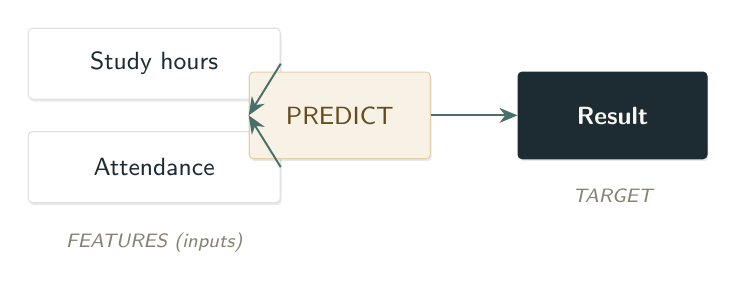
\begin{tikzpicture}[node distance=0.4cm]
        \node[card, minimum width=3.2cm] (f1) {Study hours};
        \node[card, below=of f1, minimum width=3.2cm] (f2) {Attendance};
        \node[warm, right=1.2cm of $(f1)!0.5!(f2)$, minimum width=2.3cm,
              minimum height=1.1cm] (t) {PREDICT};
        \node[solid, right=1.1cm of t, minimum width=2.4cm, minimum height=1.1cm]
          (tg) {Result};
        \foreach \n in {f1,f2} \draw[flow] (\n.east) -- (t.west);
        \draw[flow] (t) -- (tg);
        \node[tag, below=0.25cm of f2] {FEATURES (inputs)};
        \node[tag, below=0.25cm of tg] {TARGET};
      \end{tikzpicture}
      \vspace{0.6em}
      \begin{center}
      \begin{minipage}{6.4cm}
        {\footnotesize\color{ink}
         The \textbf{features} are what we feed in.\\
         The \textbf{target} is what we predict.\\[4pt]
         {\color{stone}A bigger, cleaned class of 14 --- too small to trust,
          big enough to see every step.}}
      \end{minipage}
      \end{center}
    \end{column}
  \end{columns}
  \note{%
    Reuse the exact words from Lecture 2: features are the input columns,
    the target is the column we want to predict. Here features are Study hours
    and Attendance; the target is Result (Pass/Fail).\\
    Note we need a target that is already filled in for past students --- that is
    how the model learns. You cannot learn to predict pass/fail from students
    whose result you never recorded.\\
    Be honest about the data: 14 students is still tiny (Lecture 1: five students
    prove nothing). We use 14 so the whole thing fits on screen. Real models
    learn from thousands. Everything we do would be identical at that scale.}
\end{frame}

%=====================================================================
% SLIDE 6 -- THE ONE HONEST TRICK: TRAIN vs TEST             (4 min)
%=====================================================================
\setkick{Part 2 \textperiodcentered\ Build the model}
\begin{frame}{The one honest trick: hide some students}
  \vspace{0.3em}
  \begin{center}
  \fitin{13.8cm}{3.6cm}{%
  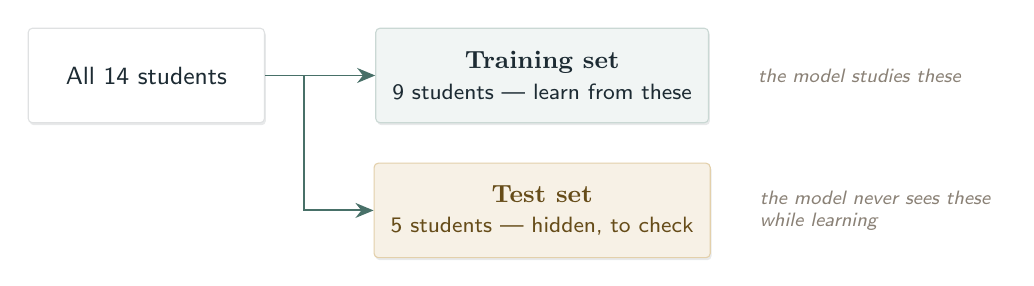
\begin{tikzpicture}[node distance=0.9cm]
    \node[card, minimum width=3.0cm, minimum height=1.2cm] (all)
      {All 14 students};
    \node[soft, right=1.4cm of all, minimum width=3.6cm, minimum height=1.2cm]
      (tr) {{\rmfamily\bfseries Training set}\\ {\footnotesize 9 students --- learn from these}};
    \node[warm, below=0.5cm of tr, minimum width=3.6cm, minimum height=1.2cm]
      (te) {{\rmfamily\bfseries Test set}\\ {\footnotesize 5 students --- hidden, to check}};
    \draw[flow] (all.east) -- ++(0.5,0) |- (tr.west);
    \draw[flow] (all.east) -- ++(0.5,0) |- (te.west);
    \node[tag, right=0.5cm of tr, text width=3.0cm] {the model studies these};
    \node[tag, right=0.5cm of te, text width=3.0cm] {the model never sees these while learning};
  \end{tikzpicture}}
  \end{center}
  \vspace{0.7em}
  \statement[12.8cm]{\fontsize{17}{23}\selectfont
    Teach the model on most students.\\
    Keep a few \textbf{hidden} to test if it really learned.}
  \note{%
    The single most important idea in the lecture --- go slowly.\\
    Analogy they feel in their bones: a teacher who gives you the exact exam
    questions to practise cannot tell if you \emph{learned} or just
    \emph{memorised}. To test real learning, the exam must have questions you
    have not seen.\\
    Same for a model: if we test it on the very students it learned from, of
    course it looks perfect --- it memorised them. So we hide some students (the
    test set), train on the rest, then check the model on the hidden ones. That
    is the only honest way to ask ``did it actually learn?''\\
    We will hide 5 of our 14 and train on 9.}
\end{frame}

%=====================================================================
% SLIDE 7 -- SET IT UP (features, target, split)             (4 min)
%=====================================================================
\begin{frame}{Set it up}
  \vspace{0.2em}
  \begin{center}
  \fitin{13.8cm}{4.6cm}{%
  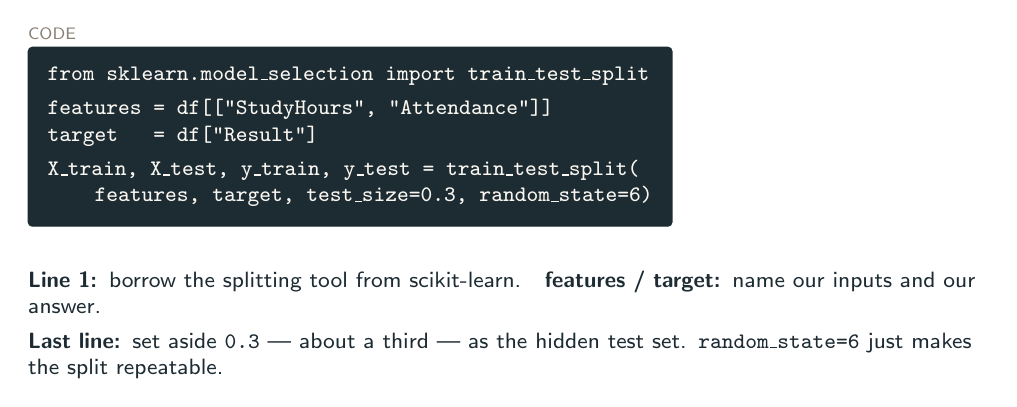
\begin{tikzpicture}
    \node[code, anchor=north west] (c) at (0,0)
      {from sklearn.model\_selection import train\_test\_split\\[3pt]
       features = df[["StudyHours", "Attendance"]]\\
       target\ \ \ = df["Result"]\\[3pt]
       X\_train, X\_test, y\_train, y\_test = train\_test\_split(\\
       \ \ \ \ features, target, test\_size=0.3, random\_state=6)};
    \lab{c}{CODE}
    \node[anchor=north west, text width=12.2cm, align=left, font=\footnotesize,
          text=ink, inner sep=0pt] at ([yshift=-0.55cm]c.south west)
      {\textbf{Line 1:} borrow the splitting tool from scikit-learn.\quad
       \textbf{features / target:} name our inputs and our answer.\\[3pt]
       \textbf{Last line:} set aside \cd{0.3} --- about a third --- as the hidden
       test set. \cd{random\_state=6} just makes the split repeatable.};
  \end{tikzpicture}}
  \end{center}
  \vspace{0.4em}
  \begin{center}
  
\begin{tikzpicture}[node distance=0.6cm]
    \node[soft, minimum width=4.2cm, font=\small] (a)
      {\cd{X\_train, y\_train} --- 9 students};
    \node[warm, right=of a, minimum width=4.2cm, font=\small] (b)
      {\cd{X\_test, y\_test} --- 5 students};
  \end{tikzpicture}
  \end{center}
  \note{%
    Read it as sentences, not code. ``Borrow the splitting tool.'' ``The features
    are these two columns; the target is Result.'' ``Split them into a training
    part and a testing part, keeping 30\% for testing.''\\
    \texttt{random\_state=6} is the only mysterious bit --- say plainly it just
    fixes which students land in which pile, so everyone running this gets the
    same split. Nothing deep.\\
    Result: four names, two piles. 9 students to learn from, 5 hidden away. We
    have not built anything yet --- just prepared the two piles.}
\end{frame}

%=====================================================================
% SLIDE 8 -- TEACH IT, THEN TEST IT                          (4 min)
%=====================================================================
\begin{frame}{Teach it, then test it}
  \vspace{0.2em}
  \begin{center}
  \fitin{13.8cm}{4.7cm}{%
  \begin{tikzpicture}
    \node[code, anchor=north west] (c) at (0,0)
      {from sklearn.tree import DecisionTreeClassifier\\[3pt]
       model = DecisionTreeClassifier()\\
       model.fit(X\_train, y\_train)\ \ \ \ \ \ \textcolor{paper!55}{\# learn}\\[3pt]
       model.score(X\_test, y\_test)\ \ \ \ \ \ \textcolor{paper!55}{\# check}};
    \lab{c}{CODE}
    \node[out, anchor=north west, font=\ttfamily\Large, inner sep=9pt] (o)
      at ([xshift=1.0cm]c.north east) {0.80};
    \lab{o}{OUTPUT}
    \node[anchor=north west, text width=3.3cm, align=left, font=\footnotesize,
          text=stone] at ([yshift=-0.3cm]o.south west)
      {it got \textbf{4 of 5}\\ hidden students right};
  \end{tikzpicture}}
  \end{center}
  \vspace{0.4em}
  \begin{center}
  \begin{minipage}{12.8cm}\centering
    {\normalsize\color{ink}
     \cd{.fit()} is the model \textbf{learning} from the training students.\quad
     \cd{.score()} is its mark on the \textbf{hidden} ones.}
  \end{minipage}
  \end{center}
  \note{%
    Three lines, three ideas.\\
    \texttt{DecisionTreeClassifier()} --- ``give me an empty model of this kind''.
    Do not explain the name yet; the next slide shows what it learned.\\
    \texttt{model.fit(X\_train, y\_train)} --- this is the learning step. ``Look
    at these 9 students and their results, and work out the pattern.'' This one
    line is the whole of ``machine learning''.\\
    \texttt{model.score(X\_test, y\_test)} --- ``now mark yourself on the 5
    hidden students''. It got 0.80 --- four right out of five. Celebrate it, then
    immediately ask: which one did it get wrong? That is the next slide, and it
    is the interesting one.}
\end{frame}

%=====================================================================
% SLIDE 9 -- READING THE TEST RESULT                         (3 min)
%=====================================================================
\begin{frame}{What it got right --- and wrong}
  \vspace{0.3em}
  \begin{center}
  \fitin{13.8cm}{4.2cm}{%
    \sffamily\small\renewcommand{\arraystretch}{1.3}%
    \setlength{\tabcolsep}{10pt}%
    \begin{tabular}{llrrll}
      \arrayrulecolor{terra}\toprule
      & \textbf{Student} & \textbf{Study} & \textbf{Att.} &
        \textbf{Actual} & \textbf{Model said}\\
      \arrayrulecolor{ink!20}\midrule
      & Oishi  & 3 & 85 & \pass & \pass \ {\footnotesize\color{sage!45!black}right}\\
      & Karim  & 1 & 55 & \fail & \fail \ {\footnotesize\color{sage!45!black}right}\\
      & Lima   & 6 & 85 & \pass & \pass \ {\footnotesize\color{sage!45!black}right}\\
      & Nusrat & 7 & 90 & \pass & \pass \ {\footnotesize\color{sage!45!black}right}\\
      \rowcolor{terra!10}
      & Fahim  & 8 & 90 & \fail & \pass \ {\footnotesize\color{terra}\textbf{wrong}}\\
      \bottomrule
    \end{tabular}}
  \end{center}
  \vspace{0.5em}
  \begin{center}
  \begin{minipage}{12.6cm}\centering
    {\normalsize\color{ink}
     Fahim studied 8 hours with 90\% attendance --- he \textit{looked} like a
     pass. The model guessed Pass. He actually failed.}
  \end{minipage}
  \end{center}
  \note{%
    This is the honest heart of the lecture --- do not rush past it.\\
    Four of the five hidden students: the model matched reality. Good.\\
    Fahim is the lesson. On paper he looks like a strong student --- lots of
    study, high attendance --- so the model, following the pattern, said Pass.
    But he failed, for a reason not in our two columns (illness, stress,
    a hard course --- we do not know). The model only knows what it was given.\\
    Say it plainly: a model is a very good guess, never a certainty. It will be
    wrong sometimes, and the wrong cases are often the most human ones. Hold
    Fahim --- he comes back when we talk about the cost of a mistake.}
\end{frame}

%=====================================================================
% SLIDE 10 -- USE IT ON A NEW STUDENT                        (3 min)
%=====================================================================
\begin{frame}{Now use it on a brand-new student}
  \vspace{0.2em}
  \begin{center}
  \fitin{13.8cm}{4.4cm}{%
  \begin{tikzpicture}
    % new student 1
    \node[code] (c1) {model.predict([[6, 85]])};
    \lab{c1}{A NEW STUDENT: 6 HOURS, 85\% ATTENDANCE}
    \node[out, anchor=west, inner sep=7pt] (o1) at ([xshift=0.7cm]c1.east)
      {['\pass']};
    \draw[flow] (c1.east) -- (o1.west);
    % new student 2
    \node[code, anchor=north west] (c2) at ([yshift=-0.9cm]c1.south west)
      {model.predict([[2, 55]])};
    \lab{c2}{ANOTHER: 2 HOURS, 55\% ATTENDANCE}
    \node[out, anchor=west, inner sep=7pt] (o2) at ([xshift=0.7cm]c2.east)
      {['\fail']};
    \draw[flow] (c2.east) -- (o2.west);
    \node[anchor=north west, text width=11.0cm, align=left, font=\footnotesize,
          text=stone, inner sep=0pt] at ([yshift=-0.7cm]c2.south west)
      {These two students are not in the table at all. The model has never seen
       them --- yet it gives an answer in an instant. This is the point of a
       model: it works on people it was never shown.};
  \end{tikzpicture}}
  \end{center}
  \vspace{0.3em}
  \statement[12.6cm]{\fontsize{16}{22}\selectfont
    The pattern it learned now works on \textbf{anyone} ---\\
    one student or five thousand.}
  \note{%
    The payoff moment --- this is what all the work was for.\\
    We hand the model a student described only by study hours and attendance,
    someone not in our data. \texttt{predict} returns a guess instantly: the
    6-hour, 85\% student --- Pass; the 2-hour, 55\% student --- Fail.\\
    Connect to day one: this is precisely ``how YouTube knows'' --- it learned a
    pattern from millions of past viewers and applies it to you, a new viewer.
    Same idea, different data.\\
    Remind them gently: these are guesses, not verdicts. Useful for deciding whom
    to offer help, never for deciding whom to give up on.}
\end{frame}

%=====================================================================
% SLIDE 11 -- WHAT DID IT LEARN?                             (3 min)
%=====================================================================
\setkick{Part 3 \textperiodcentered\ Trust and judgement}
\begin{frame}{What did the model actually learn?}
  \vspace{0.3em}
  \begin{center}
  \fitin{13.8cm}{3.9cm}{%
  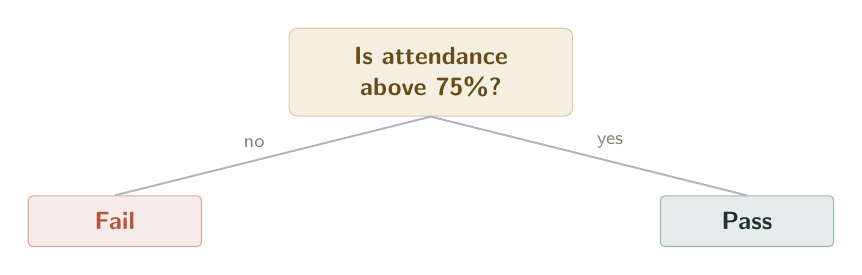
\begin{tikzpicture}[node distance=1.0cm and 1.4cm]
    \node[qnode] (q) {Is attendance\\ above 75\%?};
    \node[leafF, below left=1.0cm and 1.1cm of q] (f) {Fail};
    \node[leafP, below right=1.0cm and 1.1cm of q] (p) {Pass};
    \draw[branch] (q.south) -- (f.north)
      node[midway, above left=-1pt, font=\scriptsize, text=stone] {no};
    \draw[branch] (q.south) -- (p.north)
      node[midway, above right=-1pt, font=\scriptsize, text=stone] {yes};
  \end{tikzpicture}}
  \end{center}
  \vspace{0.4em}
  \begin{center}
  \begin{minipage}{12.6cm}\centering
    {\normalsize\color{ink}
     The model is just a \textbf{question}, learned from the data. It discovered
     that \textbf{attendance} was the strongest clue --- the very warning sign
     Lecture 1 predicted.}
  \end{minipage}
  \end{center}
  \note{%
    A ``decision tree'' is nothing more than a flowchart of yes/no questions ---
    exactly the yes/no questions we asked in Lecture 3 when we wrote
    \texttt{df["CGPA"] <= 4.0}. The difference: here the computer \emph{chose}
    the question itself, from the data.\\
    Our model learned one clean question: is attendance above 75\%? Above --
    guess Pass; below -- guess Fail. That is why it misread Fahim (90\%
    attendance, but failed anyway).\\
    The lovely full-circle moment: in Lecture 1 we said attendance would probably
    be the strongest early warning sign. We did not tell the model that --- it
    worked it out on its own. That is the whole promise of the field in one
    picture.}
\end{frame}

%=====================================================================
% SLIDE 12 -- CAN WE TRUST IT? THE COST OF BEING WRONG       (4 min)
%=====================================================================
\begin{frame}{A wrong guess has a cost}
  \vspace{0.3em}
  \begin{center}
  \fitin{13.8cm}{3.7cm}{%
  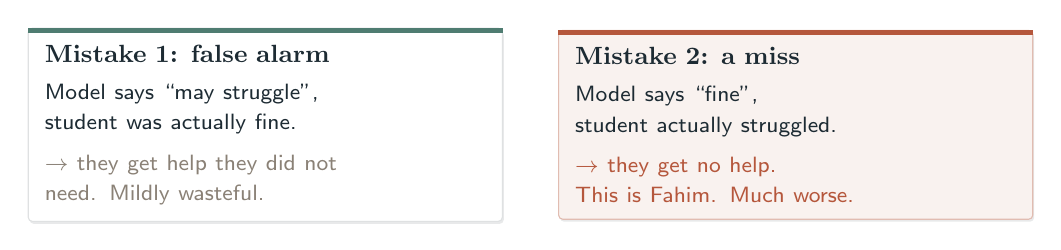
\begin{tikzpicture}[node distance=0.7cm]
    \node[card, text width=5.6cm, minimum height=2.2cm, align=left] (a)
      {{\rmfamily\bfseries Mistake 1: false alarm}\\[4pt]
       {\footnotesize Model says ``may struggle'',\\ student was actually fine.}\\[5pt]
       {\color{stone}\footnotesize $\rightarrow$ they get help they did not\\ need. Mildly wasteful.}};
    \node[card, text width=5.6cm, minimum height=2.2cm, align=left,
          right=of a, fill=terra!8, draw=terra!40] (b)
      {{\rmfamily\bfseries Mistake 2: a miss}\\[4pt]
       {\footnotesize Model says ``fine'',\\ student actually struggled.}\\[5pt]
       {\color{terra}\footnotesize $\rightarrow$ they get no help.\\ This is Fahim. Much worse.}};
    \accentbar{a}{sage}\accentbar{b}{terra}
  \end{tikzpicture}}
  \end{center}
  \vspace{0.5em}
  \statement[12.8cm]{\fontsize{16}{22}\selectfont
    ``80\% accurate'' is not the whole story.\\
    \textbf{Which} mistakes it makes matters more.}
  \note{%
    Return to Lecture 1's two kinds of error, now with a face on each.\\
    Mistake 1, a false alarm: we offer help to a student who was fine. A little
    wasted effort, no harm done.\\
    Mistake 2, a miss: we tell the teacher a struggling student is fine, so
    nobody reaches out. That is Fahim --- the model said Pass, he failed, and in
    a real system he would have slipped through. Much more costly.\\
    So a single accuracy number hides the important question: of its mistakes,
    how many are the dangerous kind? For helping students, you would rather the
    model raise a few false alarms than miss someone. Accuracy alone never tells
    you that --- human judgement decides which error you can live with.}
\end{frame}

%=====================================================================
% SLIDE 13 -- A WORD ON FAIRNESS                             (3 min)
%=====================================================================
\begin{frame}{A model only repeats its data}
  \vspace{0.4em}
  \begin{center}
  \fitin{13.8cm}{3.0cm}{%
  
\begin{tikzpicture}[node distance=1.0cm]
    \node[card, minimum width=3.4cm, minimum height=1.1cm] (d) {Past data};
    \node[warm, right=of d, minimum width=3.0cm, minimum height=1.1cm] (m) {Model};
    \node[solid, right=of m, minimum width=3.4cm, minimum height=1.1cm] (p)
      {Its predictions};
    \draw[flow] (d) -- (m);
    \draw[flow] (m) -- (p);
    \node[tag, below=0.3cm of d, text width=3.4cm] {if this is biased\ldots};
    \node[tag, below=0.3cm of p, text width=3.4cm] {\ldots so is this};
  \end{tikzpicture}}
  \end{center}
  \vspace{0.6em}
  \begin{center}
  \begin{minipage}{12.6cm}
    {\normalsize\color{ink}
     A model copies the patterns in the data it was given. Feed it unfair or
     biased history, and it will repeat that unfairness --- confidently.}\\[6pt]
    {\color{stone}\footnotesize So: use features that are \textit{fair} and
     relevant (study, attendance --- not religion, gender, or home district),
     and never let a prediction be the final word about a person.}
  \end{minipage}
  \end{center}
  \note{%
    Short but important --- the course has raised ethics since Lecture 1, so close
    the loop.\\
    The core idea, in their words from Lecture 1: ``the model does not know
    anything; it only repeats patterns it has seen''. If those patterns are
    unfair, the model launders the unfairness into something that looks
    objective because ``the computer said so''.\\
    Two rules of thumb: choose features that are fair and actually relevant; and
    keep a human in the loop --- a prediction flags who might need a
    conversation, it never decides someone's fate. This is what separates a
    responsible data scientist from a careless one.}
\end{frame}

%=====================================================================
% SLIDE 14 -- THE WHOLE WORKFLOW, DONE                       (3 min)
%=====================================================================
\setkick{Part 4 \textperiodcentered\ Closing the course}
\begin{frame}{You have now done the whole workflow}
  \vspace{0.5em}
  \begin{center}
  \fitin{13.6cm}{3.4cm}{%
  
\begin{tikzpicture}[node distance=0.42cm]
    \node[solid, minimum width=2.0cm] (q) {ASK};
    \node[soft, right=of q, minimum width=2.0cm] (co) {COLLECT};
    \node[soft, right=of co, minimum width=2.0cm] (cl) {CLEAN};
    \node[soft, right=of cl, minimum width=2.0cm] (ex) {EXPLORE};
    \node[soft, right=of ex, minimum width=2.0cm] (pr) {PREDICT};
    \node[warm, right=of pr, minimum width=2.1cm, fill=terra!14, draw=terra!55,
          text=terra] (de) {DECIDE};
    \foreach \a/\b in {q/co,co/cl,cl/ex,ex/pr,pr/de} \draw[flow] (\a) -- (\b);
  \end{tikzpicture}}
  \end{center}
  \vspace{1.0em}
  \statement[13.0cm]{\fontsize{18}{24}\selectfont
    You can take a question, get data, clean it,\\
    explore it, and make a first prediction.\\[4pt]
    {\normalsize\color{stone} That is the entire journey of Lecture 1 --- done by you.}}
  \note{%
    The ``we made it'' slide. Put the Lecture 1 workflow back up, now all lit.
    Walk it once, naming the lecture that taught each box.\\
    Say it directly and warmly: on day one this diagram was a promise and it
    looked hard. Today every box is something they have actually done with their
    own hands on a real file. The last box, Decide, is the human one --- the
    prediction informs a decision, a person makes it.\\
    This is the emotional peak of the course --- let it land before the recap.}
\end{frame}

%=====================================================================
% SLIDE 15 -- FIVE THINGS YOU CAN NOW DO                     (2 min)
%=====================================================================
\begin{frame}{Five things you can now do}
  \vspace{0.6em}
  \begin{center}
  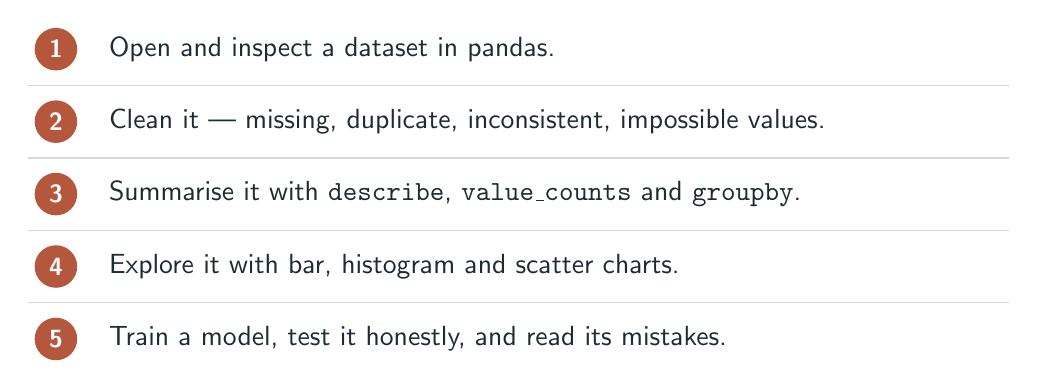
\begin{tikzpicture}[x=1cm,y=1cm]
    \foreach \i/\txt [count=\n] in {%
      1/{Open and inspect a dataset in pandas.},
      2/{Clean it --- missing, duplicate, inconsistent, impossible values.},
      3/{Summarise it with \cd{describe}, \cd{value\_counts} and \cd{groupby}.},
      4/{Explore it with bar, histogram and scatter charts.},
      5/{Train a model, test it honestly, and read its mistakes.}}{%
      \pgfmathsetmacro{\yy}{-0.92*\i}
      \node[num, minimum size=5.4mm, font=\small\bfseries] at (0,\yy) {\i};
      \node[anchor=west, font=\normalsize, text=ink, text width=11.6cm]
        at (0.55,\yy) {\txt};
      \ifnum\i<5\relax \draw[hair] (-0.35,\yy-0.46) -- (12.1,\yy-0.46);\fi}
  \end{tikzpicture}
  \end{center}
  \vspace{0.4em}
  \begin{center}{\color{stone}\normalsize
    Five lectures ago, none of this was on the table. Every one of these is a
    real skill.}
  \end{center}
  \note{%
    Do not read all five --- let them read, and pause on number 5. Five weeks ago
    ``train a model'' sounded like something only experts did; now they have done
    it.\\
    Tell them honestly what comes next if they continue: more models, more data,
    better ways to measure --- but the shape never changes. Everything is still
    this one workflow. They already own the map.\\
    This is the confidence slide. Mean it.}
\end{frame}

%=====================================================================
% SLIDE 16 -- CLOSING  (dark)
%=====================================================================
\begin{darkframe}
  \vfill
  \begin{center}
    {\sffamily\fontsize{8}{10}\selectfont\color{terra}\lsstyle
     WHERE YOU STARTED, AND WHERE YOU ARE NOW}\\[1.3em]
    
\begin{tikzpicture}
      \node[inner sep=0pt] (t)
        {\parbox{13.2cm}{\centering\rmfamily\fontsize{21}{28}\selectfont
         \color{paper} You began by asking how YouTube\\
         knew what to show you.\\[8pt]
         {\color{ochre}\bfseries Now you could build the idea behind it.}}};
      \fill[terra] ([xshift=-0.6cm]t.north west) rectangle
                   ([xshift=-0.47cm]t.south west);
    \end{tikzpicture}\\[1.6em]
    {\color{paper!65}\large Thank you. This is the end of the course ---
     and the start of what you can do with data.}
  \end{center}
  \vfill
  \note{%
    Closing slide --- keep it short, warm, and a little proud of them.\\
    Bring back the very first question of Lecture 1: how does YouTube know what
    to show you? On day one it was a mystery. Today they understand the machine
    behind it --- data, cleaned and explored, a pattern learned, a prediction
    made.\\
    Thank them genuinely, especially the ones who arrived sure this was not for
    them. Invite them to keep a dataset of something they care about and try the
    workflow on it. End on the final line and let the room clap.}
\end{darkframe}

\end{document}
